\documentclass{minimal}

\usepackage{tikz}
\usetikzlibrary{arrows,shapes,decorations,positioning,
				decorations.pathmorphing,decorations.pathreplacing,
				automata,backgrounds,
				petri,topaths,trees,
				fit,circuits.ee.IEC}	%To use diverse features from tikz		

\begin{document}
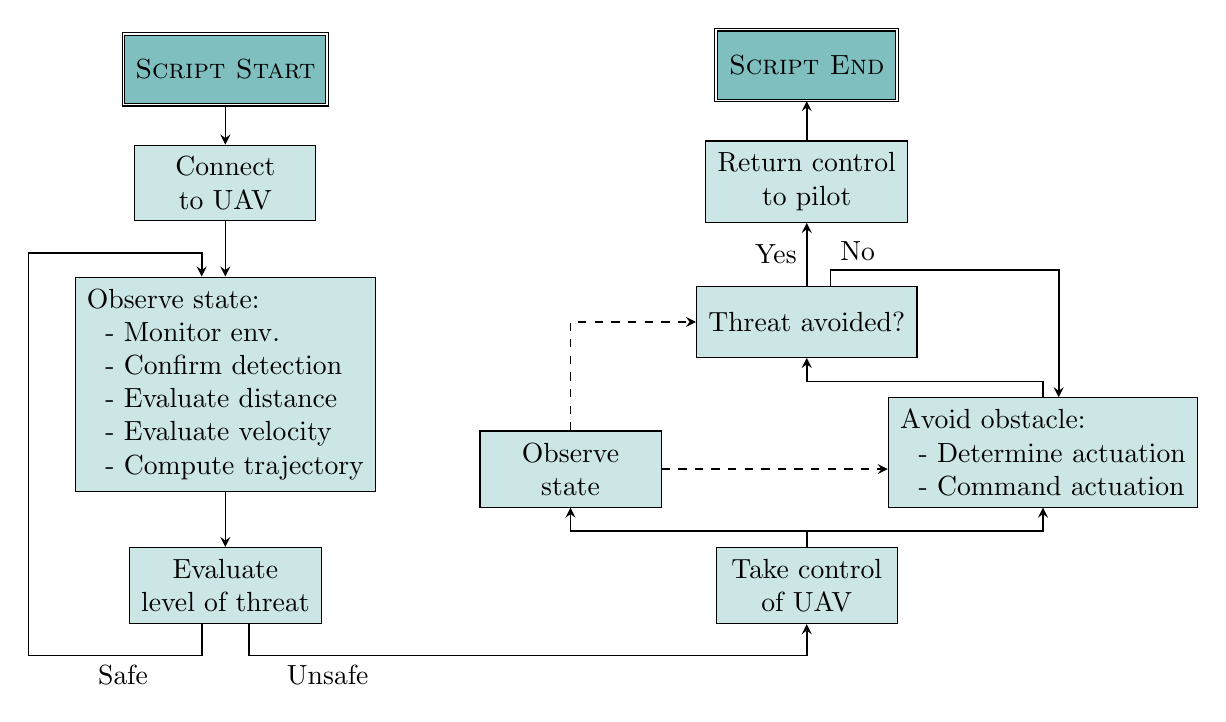
\begin{tikzpicture}

	\tikzstyle{function}=[rectangle,fill=teal!20,draw,
		minimum width=2.3cm,minimum height=0.9cm,
		node distance=0.7cm,
		align=center,inner sep=1.5mm]
	\tikzstyle{arrow}=[-stealth,semithick]

	\node[function,fill=teal!50,double](start){\scshape Script Start};
	\node[function,below=0.5cm of start](connect){Connect\\ to UAV};
	\node[function,below=of connect,align=left](observe){Observe state:\\~~- Monitor env.\\~~- Confirm detection\\~~- Evaluate distance\\~~- Evaluate velocity\\~~- Compute trajectory};
	\node[function,below=of observe](threat){Evaluate\\ level of threat};
	\coordinate (coordloop1) at ($(threat.south)+(-2.5cm,-4mm)$);
	\coordinate (coordloop2) at ($(observe.north)+(-3mm,3mm)$);
	\node[function,right=5cm of threat](take){Take control\\ of UAV};
	\coordinate (coordtake) at ($(take.south)+(-2.5cm,-4mm)$);
	\node[function,above=0.5cm of take,xshift=-3cm](observemission){Observe\\ state};
	\node[function,above=0.5cm of take,xshift=3cm,align=left](avoid){Avoid obstacle:\\~~- Determine actuation\\~~- Command actuation};
	\coordinate (coordmission) at ($(take.north)+(0,0.2cm)$);
	\node[function,above=0.5cm of avoid,xshift=-3cm](avoided){Threat avoided?};
	\coordinate (coordavoid) at ($(avoided.south)+(0,-3mm)$);
	\coordinate (coordreturn) at ($(avoided.north)+(3.2cm,2mm)$);
	\node[function,above=0.8 cm of avoided](return){Return control\\ to pilot};
	\node[function,fill=teal!50,double,above=0.5cm of return](end){\scshape Script End};
	%\coordinate (coordend) at ($(end)+(0,1cm)$);

	\draw[arrow] (start) -- (connect);
	\draw[arrow] (connect) -- (observe);
	\draw[arrow] (observe) -- (threat);
	\draw[arrow] ($(threat.south)+(-3mm,0)$) |- node[below,xshift=-1cm]{Safe} (coordloop1) |- (coordloop2) -- ($(observe.north)+(-3mm,0)$);
	\draw[arrow] ($(threat.south)+(3mm,0)$) |- node[below,xshift=1cm]{Unsafe} (coordtake) -| (take);
	\draw[arrow] (take) -- (coordmission) -| (observemission);
	\draw[arrow] (take) -- (coordmission) -| (avoid);
	\draw[arrow] (avoid) |- (coordavoid) -- (avoided);
	\draw[arrow,dashed] (observemission) -- (avoid.west|-observemission);
	\draw[arrow,dashed] (observemission) |- (avoided);
	\draw[arrow] (avoided) -- node[left]{Yes} (return);
	\draw[arrow] ($(avoided.north)+(3mm,0)$) |- node[above right]{No} (coordreturn) -- (coordreturn|-avoid.north);
	\draw[arrow] (return) -- (end);

\end{tikzpicture}
\end{document}
